\section{}
% Water enters a tank of diameter �" steadily at a mass flow rate of �̇.
% An orifice at the bottom with diameter �# allows water to escape. The orifice has a rounded
% entrance, so the frictional losses are negligible. If the tank is initially empty, (a) determine the 
% maximum height that the water will reach in the tank and (b) obtain a relation for water height z
% as a function of time.

Water enters a tank of diameter $\SI{1}{\meter}$ steadily at a mass flow rate of $\dot{m}$.
An orifice at the bottom with diameter $D_0$ allows water to escape. The orifice has a rounded
entrance, so the frictional losses are negligible. If the tank is initially empty, (a) determine the
maximum height that the water will reach in the tank and (b) obtain a relation for water height $z$

\begin{figure}[h]
    \centering
    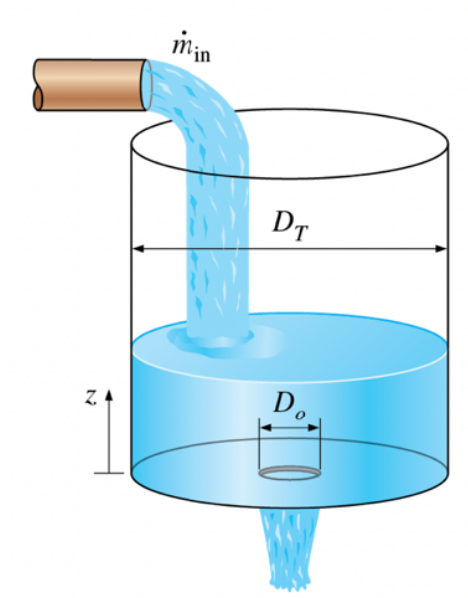
\includegraphics[width=0.4\linewidth]{Questions/Figures/Q3ProblemDiagram.png}
    \caption{Water tank}
    \label{fig:Q3ProblemDiagram}
\end{figure}

\textbf{Solution} \\
\subsection{}
Let the height of the water at the maximum height be $h$. At the maximum height, equilibrium is reached, so the mass flow rate in is equal to the mass flow rate out.

By the Bernoulli equation,
\begin{gather*}
    \underbrace{\cancel{\frac{P_1}{\rho} - \frac{P_2}{\rho}}}_{\text{Both at atm}} + \underbrace{\cancel{\frac{v_1^2}{2}}}_{\text{Sufficiently large}} - \frac{v_2^2}{2} + g(z_1 - z_2) = 0 \\
    h = \frac{v_2^2}{2g}
\end{gather*}

By the continuity equation,
\begin{align*}
    \dot{m} &= \rho A_0 v_2 \\
    \implies v_2 &= \frac{\dot{m}}{\rho A_0} \\
    &= \frac{\dot{m}}{\rho \pi D_0^2 / 4}
\end{align*}

Substituting into the Bernoulli equation,
\begin{align*}
    h &= \frac{v_2^2}{2g} \\
    &= \frac{\left(\frac{\dot{m}}{\rho \pi D_0^2 / 4}\right)^2}{2g} \\
    &= \boxed{\frac{8 \dot{m}^2}{\rho^2 \pi^2 g D_0^4}}
\end{align*}

\subsection{}
Let the height of the water at time $t$ be $z(t)$. At a given time, the exit velocity is given by the Bernoulli equation,
\begin{gather*}
    \underbrace{\cancel{\frac{P_1}{\rho} - \frac{P_2}{\rho}}}_{\text{Both at atm}} + \underbrace{\cancel{\frac{v_1^2}{2}}}_{\text{Sufficiently large}} - \frac{v_2^2}{2} + g(z_1 - z_2) = 0 \\
    \implies v_2 = \sqrt{2gz(t)}
\end{gather*}

Accumulation of mass in the tank is given by the continuity equation,
\begin{align*}
    \dot{V} &= \dot{m} - A_0 v_2 
\end{align*}
Substituting expressions for $V$, $A_0$, and $v_2$,
\begin{align*}
    \frac{d}{dt} \left(\frac{\pi D_T^2}{4} z(t)\right) &= \dot{m} - \frac{\pi D_0^2}{4} \sqrt{2gz(t)} \\
    \frac{\pi D_T^2}{4} \dot{z}(t) &= \dot{m} - \frac{\pi D_0^2}{4} \sqrt{2gz(t)} \\
\end{align*}
Observe this is a constant coefficient, first order, non-homogeneous, non-linear differential equation. I do not know how to solve this,
nor does it seem particularly useful to solve this with tools such as \texttt{ODE45}. As such, I will just box the implicit relationship.
\begin{empheq}[box=\fbox]{align*}
    \frac{\pi D_T^2}{4} \dot{z}(t) &= \dot{m} - \frac{\pi D_0^2}{4} \sqrt{2gz(t)}
\end{empheq}

% random latex that i need rendered quickly

\begin{align*}
    \theta_{wall} &= A_1 \exp(-\lambda^{2}_1 \tau) \\
    \implies \tau &= \frac{-\ln \left(\frac{\theta_{wall}}{A_1}\right)}{\lambda^{2}_1}  \\
    \implies t &= \frac{L^2}{\alpha} \frac{-\ln \left(\frac{\theta_{wall}}{A_1}\right)}{\lambda^{2}_1} \\
\end{align*}
